\chapter{Interattivit\`a}\label{ch:interactivity}

Un modo semplice per aumentare l'accuratezza del programma \`e renderlo interattivo chiedendo aiuto all'utente per riconoscere le parole. Questo potrebbe sembrare insensato, visto che lo scopo del software \`e riconoscere i grafemi in maniera automatica, tuttavia non \`e cos\`i visto che il programma continuerebbe a fare la maggior parte del lavoro. Infatti, il programma fa tutto il processo descritto nei primi capitoli, fino a individuare le varie lettere e anche scartare quelle che sono molto diverse dal riferimento. L'unica cosa che viene chiesta all'utente \`e individuare i grafemi che corrispondono al riferimento scegliendo fra i pochi che rimangono.

\section{Interfaccia interattiva}

Per quanto riguarda l'interfacciamento con l'utente, questo avviene in modo molto semplice: si apre una finestra che chiede all'utente se la lettera mostrata \`e corretta che, quando l'utente ha risposto, si richiude per mostrarne un'altra. In questo modo l'utente deve fare una sola azione (premere un tasto) per ogni grafema mostrato, quindi viene ridotta al minimo la parte di lavoro non automatizzata.

L'interfaccia che vede l'utente \`e quella di figura \ref{fig:gui}. Nella prima riga c'\`e il comando in cui si dice di premere il tasto \emph{y} (``yes'') se la lettera \`e quella che si sta cercando o il tasto \emph{n} (``no'') in caso contrario. Viene anche mostrato l'indice di Jaccard relativo alla lettera per avere un'informazione aggiuntiva.

\begin{figure}
    \centering
    \frame{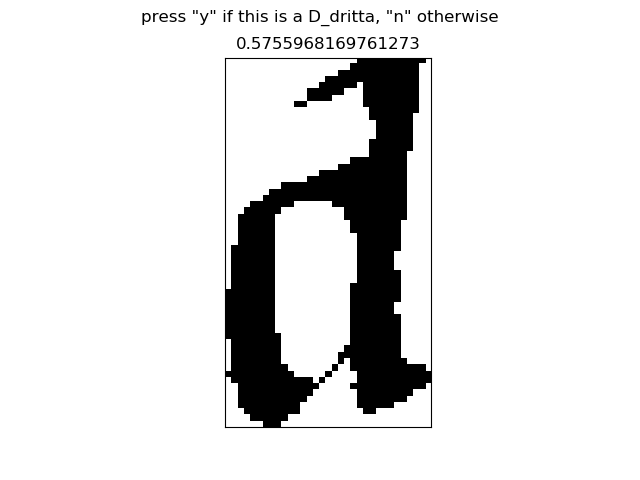
\includegraphics[width=.8\textwidth]{figures/gui.png}}
    \caption{L'interfaccia grafica sviluppata. In alto le indicazioni e l'indice di Jaccard nella seconda riga.}
    \label{fig:gui}
\end{figure}

\section{Interattivit\`a limitata}

Nel caso di documenti molto lunghi, comprendenti dunque molte pagine, chiedere conferma all'utente per ogni lettera, significherebbe chiedergli troppo lavoro. Tuttavia ci\`o non significa che l'interattivit\`a non sia una buona idea.

La soluzione consiste nell'integrare una parte interattiva con una parte completamente automatica. In pratica, durante la parte interattiva si raccolgono nuovi riferimenti che verranno poi utilizzati nella parte completamente automatica. Questo significa che nel primo round verranno selezionate soltanto alcune lettere. Per scegliere le lettere da usare nel primo round \`e necessario usare un generatore di numeri casuali, altrimenti si possono avere effetti indesiderati (se, ad esempio, analizziamo solamente una pagina potrebbe succedere che la grafia di pagine successive sia diversa da quella della pagina selezionata).

\subsection{Tipi di media}

Una volta che abbiamo l'insieme di riferimenti trovati in maniera casuale e interattiva, possiamo calcolare, per ogni nuova lettera, gli indici di Jaccard relativi a ciascun riferimento. Adesso per\`o dobbiamo trovare un modo per passare da tanti valori ad uno solo indicativo di tutti.

Ci\`o che stiamo cercando \`e una funzione che faccia da media. Potremmo pensare di usare la media aritmetica, ma questa non ha certe propriet\`a che stiamo cercando. Infatti vogliamo che la funzione restituisca 1 quando almeno uno degli elementi \`e 1. Questo perch\'e il fatto che uno dei valori sia 1 equivale a dire che la lettera che stiamo testando \`e identica ad un riferimento e perci\`o \`e corretta sicuramente.

A questo punto potremmo pensare di usare come media la funzione \emph{max}, che restituisce il massimo dei valori in ingresso. Questa funzione ha infatti la propriet\`a di cui abbiamo parlato prima: se 1 \`e fra i valori in ingresso, allora \emph{max} restituir\`a sicuramente 1 (ricordiamo che i valori di ingresso sono indici di Jaccard e perc\`o sono sempre compresi fra 0 e 1 inclusi). Tuttavia, neanche questa funzione \`e adatta, poich\'e non tiene conto dei valori pi\`u bassi. Questo \`e un problema perch\'e passare da una lista di valori $(\frac{1}{2})$ a $(\frac{1}{2}, \frac{1}{4})$ deve far diminuire l'indice risultante.

Dopo queste considerazioni arriviamo alla seguente formula.
\begin{equation*}
    1 - \prod_{0\leq i < n} (1-x_i)
\end{equation*}
In cui $n$ \`e il numero di valori in ingresso. Con questa funzione tutti i valori contribuiscono al risultato finale a meno che uno dei valori sia 1, in qual caso il risultato \`e 1. Ancora per\`o non \`e perfetta come funzione, infatti se prendo $A = ( \frac{1}{2}, \frac{1}{2} )$, il risultato non \`e $\frac{1}{2}$ come sarebbe ovvio aspettarsi, ma $\frac{3}{4}$.

Dopo un ultimo ritocco alla formula, si arriva alla forma seguente.
\begin{equation*}
    1 - \sqrt[n]{\prod_{0\leq i < n} (1-x_i)}
\end{equation*}
Questa ha tutte le propriet\`a della funzione precedente e in pi\`u, se tutti i valori sono uguali, restituisce il valore in ingresso.

\section{Confronto con modalit\`a non interattiva}

Per verificare se l'introduzione di interattivit\`a ha aiutato il programma dobbiamo confrontarne i risultati con quelli che ottenevamo senza interattivit\`a. Nelle figure \ref{fig:graph_total_static}, \ref{fig:graph_total_baricenter} e \ref{fig:graph_total_inertia} sono mostrati i grafici precision recall per le varie modalit\`a.

\begin{figure}
    \centering
    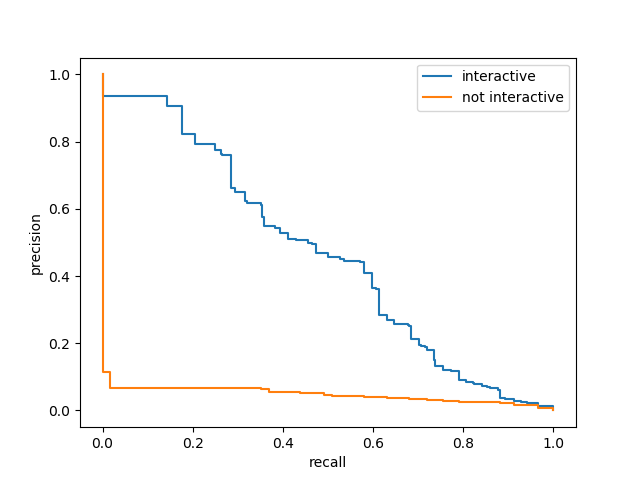
\includegraphics[width=.9\textwidth]{figures/graphs/totalstaticFalse.png}
    \caption{Curve precision recall con e senza interattivit\`a, metodo centrale.}
    \label{fig:graph_total_static}
\end{figure}

\begin{figure}
    \centering
    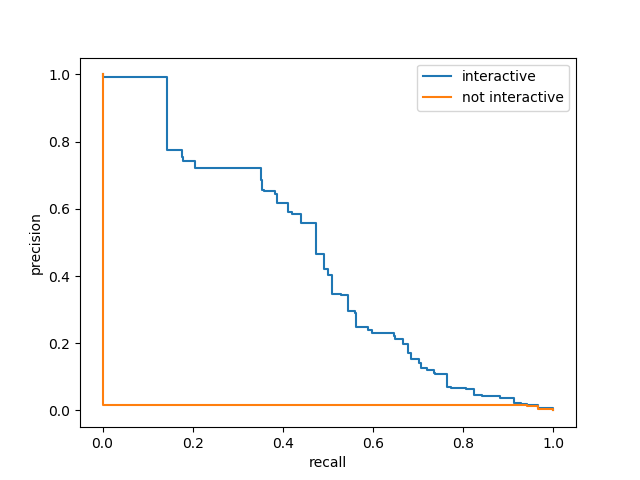
\includegraphics[width=.9\textwidth]{figures/graphs/totalbaricenterFalse.png}
    \caption{Curve precision recall con e senza interattivit\`a, metodo del baricentro.}
    \label{fig:graph_total_baricenter}
\end{figure}

\begin{figure}
    \centering
    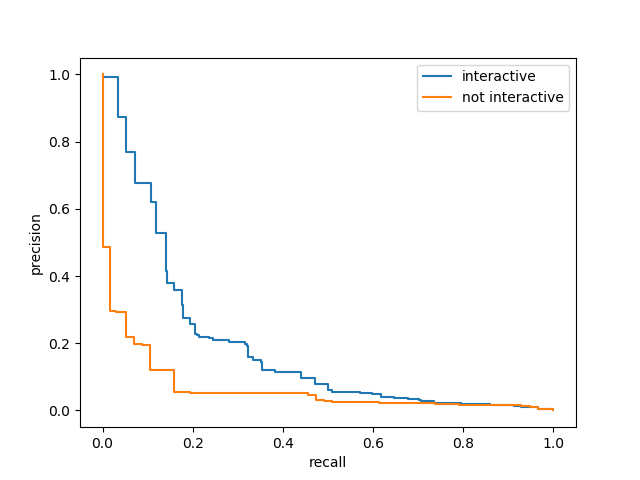
\includegraphics[width=.9\textwidth]{figures/graphs/totalinertiaFalse.png}
    \caption{Curve precision recall con e senza interattivit\`a, metodo inerziale.}
    \label{fig:graph_total_inertia}
\end{figure}

Come si nota nelle figure, le curve relative alla non interattivit\`a sono diverse rispetto a quelle del capitolo precedente. Questo perch\'e sono state utilizzate pagine diverse per enfatizzare il punto forte dell'interattivit\`a: \`e efficace con pagine scritte con calligrafie diverse.

\`E evidente come il metodo inerziale sia il peggiore dei tre in questa modalit\`a. Infatti anche in questo caso le lettere sono tutte della stessa grandezza pi\`u o meno. Si faccia caso, per\`o, al fatto che il metodo inerziale \`e il migliore nella modalit\`a non interattiva. Questo \`e dovuto al fatto che, come avevamo predetto nella sezione \ref{ssect:jaccard}, questo metodo \`e adatto ai casi in cui le pagine hanno stili differenti e in particolare hanno lettere di dimensione variabile.

Come prima, mostriamo anche le misure delle aree sotto le curve di precision recall nella tabella \ref{tab:area_interactive}. Va ricordato che questi valori non sono deterministici come quelli del capitolo \ref{ch:experiments}, ma dipendono dalla scelta casuale delle lettere estratte e usate per l'interattivit\`a.

\begin{table}
    \centering
    \begin{tabular}{c|c|c|c}
        connettivit\`a & modalit\`a & interattivo & non interattivo  \\
        \hline
        \multirow{3}{1em}{4} & centro & 0.463 & 0.047 \\
        & baricentro & 0.448 & 0.017 \\
        & inerzia & 0.188 & 0.063 \\
        \hline
        \multirow{3}{1em}{8} & centro & 0.449 & 0.046 \\
        & baricentro & 0.391 & 0.017 \\
        & inerzia & 0.193 & 0.063 \\
    \end{tabular}
    \caption{Le aree sotto le curve precision recall per tutti i metodi interattivi testati e il confronto rispetto agli stessi metodi senza interattivit\`a.}
    \label{tab:area_interactive}
\end{table}